\section{Algorítimos de \textit{string matching} inexatos} % (fold)
\label{sec:algor_timos_de_string_matching_inexatos}

Para a busca com algorítimos de \textit{string matching} inexatos, foram considerado dois métodos distintos:

\begin{description}
	\item[Levenshtein:] Método voltado para correção de erros. Foi previamente comentado na sessão de \ref{sec:leveinstein}.
	\item[Coeficiente de Sørensen–Dice:] Método que faz de uso do conceito de autômatos de estados para agilizar a busca. Previamente apresentado na \autoref{ssub:s_rensen_dice_coefficient}.
\end{description}

Para analise de desempenho, foram coletadas 150 amostras de tempo para 10 buscas por pacotes distintos das quais metade eram de pacotes que não existiam, semelhante realizado para os \lnameref{sec:algor_timos_de_string_matching_exatos}. A \autoref{tempo_rk_kmp_std_lev_dic} retrata a mediana destes tempos.

\begin{figure}[htbp]
  \centering
  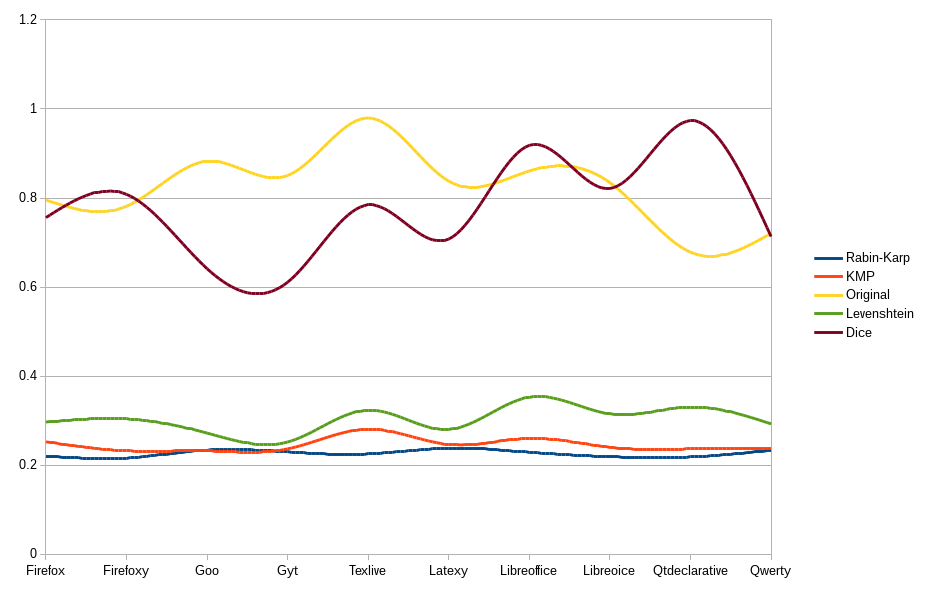
\includegraphics[width=0.95\textwidth]{figuras/tempo-rk_kmp_std_lev_dice}
  \caption{Estimativa de tempo para pacotes usando algorítimos de busca inexata}
  \label{tempo_rk_kmp_std_lev_dic}
\end{figure}

Como apresentado na primeira etapa deste trabalho\footnote{Trabalho de conclusão de curso 1: Algoritmo para Qualificação das Saídas de Buscas em
Gerenciadores de Repositórios de Distribuições Linux}, o algoritmo de \textit{Leveinstein} apresenta um dos melhores tempos para buscas inexatas de \textit{strings}. A \autoref{tempo_rk_kmp_std_lev_dic} reforça essa afirmação, ao mostrar que o tempo de resposta deste algoritmo é inferior ao tempo gasto para buscas com expressões regulares e ficando pouco acima do tempo necessário para realizar buscas exatas com o algoritmo de  \textit{Rabin-Karp}.